\chapter{Implicitación de superficies}

\section{Introducción}

Las superficies implícitas se usan en la Ciencia de Computación Gráfica desde los años 70 para modelar objetos geométricos, pero su uso e importancia han ido creciendo en años recientes ya que pueden ser usadas para describir objetos en espacios de dimensión arbitraria. En este Trabajo Fin de Máster nos centraremos en objetos de dimensión dos y tres. En muchas ocasiones, un mismo objeto matemático se puede definir de una forma particular, por tanto nos cabe preguntarnos por qué las superficies en forma implícita se han popularizado tanto. La respuesta la encontramos en que la expresión implícita de una superficie, en contraste con la definición paramétrica del de la misma, suele ser compacta, manejable y es trivial comprobar la pertenencia de un punto al objeto dado. Por ejemplo, una expresión paramétrica de la esfera unidad es
$$X(u,v) = (\cos(u)\sin(v),\sin(u)\sin(v),\cos(v)), \hspace{0.5cm} (u,v) \in [0,2\pi] \times [0,\pi],$$
mientras que su expresión en forma implícita es
$$f(x,y,z) = x^2 + y^2 + z^2 - 1.$$

Aunque hemos mencionado algunas ventajas de usar la forma implícita para la modelización y visualización de superficies, su principal debilidad es la cantidad de tiempo que necesitan para la visualización directa, por ejemplo usando Ray Tracing\cite{Groot05}. Otra de las debilidades de las superficies en forma implícita es la dificultad de controlar la forma de las superficies durante una visualización rápida en un entorno interactivo. Esto lleva a que las representaciones paramétricas sigan siendo populares hoy en día gracias a la relativamente rápida renderización que presentan.

Aún presentando estas debilidades, las superficies en forma implícita son una forma flexible de crear objetos complejos ya que ofrecen una clasificación manejable y clara de conjuntos de puntos, es decir, es fácil saber si un punto del espacio se encuentra{ \em dentro},{ \em fuera} o{ \em en} la superficie.

Además también se pueden usar para la representación de nubes de puntos. Por ejemplo, en imágenes de datos médicos y reconstrucción de objetos representados como medias de conjuntos de puntos\cite{Benedet05,Peiro06}. En \cite{Uhlir03} se describe el llamado{ \em método RBF} basado en técnicas variacionales donde, dados una serie de puntos de una superficie $S$ de la cual no conocemos su expresión, procedemos a calcular una función en forma implícita que modele una superficie $S'$ que sea una aproximación razonable de la superficie inicial e interseque a los puntos que conocemos.

\section{Descripción del problema}

Una representación implícita de una superficie $S$ se define como el conjunto de puntos $p \equiv (x,y,z) \in \mathbb{R}^3$ que son solución de la ecuación $f(p) = 0$, donde $f : \mathbb{R}^3 \to \mathbb{R}$ es una función que asigna un valor escalar a cada punto del espacio. Es decir,
$$S = \{ p \in \mathbb{R}^3 : f(p) = 0 \}.$$

Sea el sólido $A$ el espacio descrito por la preimagen de la función $f$ en $]-\infty,0]$. Por uniformidad consideraremos el siguiente criterio:
$$\begin{tabular}{l c l}
    $p \in \interior(A)$ & si & $f(p) < 0$, \\
    $p \in \partial A$ & si & $f(p) = 0$, \\
    $p \in \exterior(A)$ & si & $f(p) > 0$.
\end{tabular}$$
Donde $\interior(A)$, $\partial A$ y $\exterior(A)$ denotan el interior, frontera y exterior de $A$ respectivamente. Esto establece por medio de la vía topológica que la función implícita es negativa en el{ \em interior}, cero en la superficie, véase{ \em frontera}, y positiva en el{ \em exterior}\cite{Hart01}.

Este sistema es un estándar que se suele usar por comodidad y por ser el más común entre la literatura de este tipo de trabajos. Otros ejemplos incluyen a \cite{Uhlir03} o \cite{Blinn82} donde las funciones implícitas definidas eran positivas en el interior y negativas en el exterior del sólido, o por ejemplo \cite{Ricci73} donde eran siempre positivas y alcanzaban el valor unidad en la superficie, menos uno en el interior y mayor que uno en el exterior.

Está claro que estas definiciones no afectan al problema principal, véase que, volviendo al ejemplo de la esfera, en \cite{Uhlir03} usan lo que llaman la forma inversa que sería
$$f(x,y,z) = - x^2 - y^2 - z^2 + 1.$$

Ahora que hemos descrito las ventajas de las superficies dadas de forma implícita queremos ver los métodos para crear la representación implícita de objetos arbitrarios.

Hay infinidad de métodos para la realizar la implicitación de superficies, algunos ya los hemos mencionado como los basados en nubes de puntos y/o técnicas variacionales, pero aquí nos centraremos en los métodos de eliminación de variables que parten de expresiones paramétricas de la superficie, o parte de a superficie, para después modificarlas y así obtener una expresión implícita de ésta mediante operaciones simbólicas.

\section{Métodos de eliminación de variables}

Eliminación es una disciplina matemática para suprimir variables de sistemas de ecuaciones polinomiales. En nuestro caso este método se aplica a la parametrización de la superficie que se expresa como una sistema de ecuaciones
\begin{equation}
    \begin{tabular}{c c c}
        $x_1$ & = & $f_1(t_1, \dotso, t_m)$, \\
         & $\vdots$ & \\
        $x_n$ & = & $f_n(t_1, \dotso, t_m).$
    \end{tabular}
    \nonumber
\end{equation}
En donde las funciones $f_i$ son polinomios o funciones racionales de éstos.

El método consiste encontrar las relaciones entre las variables y, así pues, la ecuación implícita que nos expresa la misma superficie que el sistema de ecuaciones de su expresión paramétrica.

En \cite{Hoffmann93} se hace una clasificación del método de la resultante, el método de la base de Gröbner y el método de Wu-Ritt. Todos los métodos que vamos a describir tienen una propiedad común y ésta es que el resultado del algoritmo es una ecuación que puede ser utilizada por métodos de visualización directa.

\subsection{Método de la base de Gröbner}

Este método se basa en encontrar una base de Gröbner para un ideal $I$, donde éste es un conjunto de polinomios que cumple con el requisito de existencia de una base de Gröbner. La búsqueda  de una base de Gröbner reducida se basa en la búsqueda de una solución exacta de un sistema de ecuaciones polinomiales. Si el sistema de ecuaciones polinomiales tiene una solución, entonces las variables del sistema son eliminadas y el conjunto original de ecuaciones se transforma. Este nuevo conjunto de ecuaciones transformadas sí puede ser solucionado de forma sencilla.

La transformación de la expresión paramétrica en un expresión implícita puede ser resuelto de una forma satisfactoria usando una base de Gröbner de un ideal. Las parametrizaciones que tenemos como entrada pueden ser tanto polinomiales como racionales.

\subsubsection*{Ideal}

Un subconjunto $I \subset k[x_1, \dotso, x_n]$ se dice ideal en $k[x_1, \dotso, x_n]$ si se verifican las siguientes dos condiciones.
\begin{enumerate}
    \item Si $f, g \in I$, entonces $f + g \in I$.
    \item Si $f \in I$, entonces $fg \in I$ para todo $g \in k[x_1, \dotso, x_n]$.
\end{enumerate}

Sean $f_1, \dotso, f_s \in k[x_1, \dotso, x_n]$, el conjunto $I =  \left\{ \sum_{i=1}^{s} g_i f_i \ : \ g_i \in k[x_1, \dotso, x_n] \right\}$ es un ideal de $k[x_1, \dotso, x_n]$ y además es el menor ideal que contiene a los polinomios $f_1, \dotso, f_s$. El conjunto $\left\{ f_1, \dotso, f_s \right\}$ se llama conjunto generador o base del ideal $I$. 

\subsubsection*{Ordenamiento de los polinomios}

Para la computación de la base de Gröbner, necesitamos el concepto de orden monomial.

\begin{definition}
    Un orden monomial se define como un orden total sobre el conjunto de los monomios en un anillo polinomial verificando esta propiedad respecto del producto, i.e., dados dos monomios $u$ y $v$ tales que $u \leq v$ y sea $w$ otro monomio, entonces $uw \leq vw$.
\end{definition}

En el caso de una cantidad finita de variables se tiene la siguiente forma equivalente.

\begin{definition}
    Un orden sobre el conjunto de monomios en un anillo polinomial se dice monomial si se verifican las siguientes condiciones:
    \begin{itemize}
        \item El orden es total.
        \item Si $u$ es un monomio cualquiera se tiene que $1 \leq u$.
    \end{itemize}
\end{definition}

Aunque existen varios órdenes monomiales, y se pueden escoger según la situación, los más comunes son los siguientes.

\textit{Orden lexicográfico}

Dado el conjunto de monomios en $n$ variables $x_1, \dotso, x_n$ tales que establecemos que $x_1 \prec x_2 \prec \dotso \prec x_n$ el orden lexicográfico se define como
$$1 \prec x_1 \prec x_1^2 \prec \dotso \prec x_2 \prec x_1 x_2 \prec x_1^2 x_2 \prec \dotso \prec x_2^2 \prec x_1x_2^2 \prec \dotso \prec x_n \prec \dotso $$

\textit{Orden lexicográfico graduado}

A diferencia del método anterior, este método primero ordena los términos por su grado y los términos de igual grado se ordenan de manera lexicográfica. Tomando el ejemplo anterior nos quedaría:
$$1 \prec x_1 \prec x_2 \prec \dotso \prec x_n \prec x_1^2 \prec x_1 x_2 \prec x_1x_2 \prec \dotso\prec x_1x_n \prec x_2^2 \prec x_2x_3 \prec \dotso$$

\subsubsection*{Reducción polinomial}

Para calcular la base de Gröbner es importante elegir un orden $\prec$, por ello tras haberlo elegido pasamos a definir los siguientes términos.

\begin{definition}
Para cada polinomio $f(x_1, \dotso, x_n)$ se define el monomio líder como el mayor término de $f$ bajo $\prec$ con coeficientes no nulos. Se denota por $LM(f)$.
\end{definition}

\begin{remark}
El coeficiente del monomio líder se llama coeficiente líder y se denota por $LC(f)$.
\end{remark}

\begin{definition}
El término líder de un polinomio $f$ se define como el producto del monomio líder. Se denota por $LT(f)$.
\end{definition}

\begin{definition}
La cola de un polinomio $f(x_1, \dotso, x_n)$, denotado por $TT(f)$ se obtiene separando el término líder del resto del polinomio.
\end{definition}

Con las definiciones dadas se puede reescribir un polinomio $f(x_1, \dotso, x_n)$ como
$$f = LT(f) + TT(f).$$
Ahora podemos proceder a la reducción polinomial propiamente dicha.

Dados dos polinomios $f(x_1, \dotso, x_n)$ y $g(x_1, \dotso, x_m)$ se dice que $g$ reduce a un polinomio $h$ respecto de $f$ si, y sólo si, $LT(g)$ se puede eliminar mediante la resta de un múltiplo apropiado de $f$. Esta operación se denota por $g \to_f h$.
Por tanto, la reducción $g \to_f h$ es posible si, y sólo si, existe un escalar $b$ y un monomio $u$ tales que $h = g - buf$ donde $b = \frac{LC(g)}{LC(f)}$ y $u =\frac{LM(g)}{LM(f)}$.

Se dice que un polinomio $g$ se reduce respecto de un conjunto, o base, de polinomios $F = \{ f_1, \dotso, f_n \}$ si $g$ es reducible respecto de uno o más polinomios de $F$. En tal caso la reducción de un polinomio puede conducir a una secuencia de reducciones, lo que es un proceso finito. Se puede probar además que cada polinomio $g_i$ en la secuencia de reducciones y el propio polinomio $g$ es un elemento del ideal $(f_1, \dotso, f_n)$.

\subsubsection*{S-polinomios}

Este proceso que hemos llevado a cabo nos conduce al concepto de \textbf{S-polinomios}. Para dos polinomios $f$ y $g$ se define su S-polinomio como:
$$S(f,g) = \frac{x^{\gamma}}{LT(f)} \cdot f - \frac{x^{\gamma}}{LT(g)} \cdot g.$$
Donde $x^{\gamma}$ representa el máximo común divisor entre los monomios líderes de $f$ y $g$.

\subsubsection*{Base de Gröbner}

Después de escoger un orden, el conjunto $G = \{ g_1, \dotso, g_l \}$ del ideal $I$ es una base de Gröbner si
$$\langle LT(g_1), \dotso, LT(g_l) \rangle = \langle LT(I) \rangle.$$
Es decir, el conjunto $G \subset I$ es la base de Gröbner si, y sólo si, el término líder de cualquier elemento de $I$ es divisible entre $LT(g_i)$ para algún $i = 1, \dotso, l$. En consecuenia una base de Gröbner de un conjunto de polinomios es un tipo concreto de base del ideal que generan que cumple:
\begin{itemize}
    \item Todo polinomio en el ideal se reduce a cero respecto a la base.
    \item Todo polinomio tiene una única forma normal respecto de la base.
\end{itemize}

Cuando la parametrización se compone de funciones polinomiales, ésta se puede expresar como
\begin{equation}
\begin{tabular}{c c c}
$x_1$ & $=$ & $f_1(t_1, \dotso, t_m)$, \\
 & $\vdots$ &  \\
$x_n$ & $=$ & $f_n(t_1, \dotso, t_m)$.
\end{tabular}
\nonumber
\end{equation}
Donde $f_1, \dotso, f_n$ son polinomios en $K[t_1, \dotso, t_m]$ con $K$ un cuerpo.

Este sistema se puede ver como la proyección $F : K^m \to K^n$ definida por
$$F(t_1,\dotso, t_m) = (f_1(t_1,\dotso, t_m), \dotso, f_n(t_1,\dotso, t_m)).$$

Entonces, la imagen es un subconjunto de $K^n$ parametrizado por el sistema previo. Teniendo en cuenta que $F(K^m)$ no es una variedad afín, se obtiene que la solución del problema de conversión de ecuaciones paramétricas a implícitas es equivalente a encontrar la variedad mínima que contiene a $F(K^m)$, i.e., el problema de implicitación consiste en la eliminación de parámetros de la descripción paramétrica. La ecuación final contiene solo las variables $x_1, \dotso, x_n$.
\\La eliminación de variables se puede realizar calculando la base de Gröbner reducida para un ideal $I = \langle x_1 - f_1, \dotso, x_n - f_n \rangle$. Para enfrentarse a este problema solo es necesario tener en cuenta el orden $\prec$.

El segundo método es la implicitación racional, la cual puede ser expresada como
\begin{equation}
\begin{tabular}{c c c}
$x_1$ & $=$ & $\frac{f_1(t_1, \dotso, t_m)}{g_1(t_1, \dotso, t_m)}$, \\
 & $\vdots$ &  \\
$x_n$ & $=$ & $\frac{f_n(t_1, \dotso, t_m)}{g_n(t_1, \dotso, t_m)}$.
\end{tabular}
\nonumber
\end{equation}
Donde $f_1, \dotso, f_n, g_1, \dotso, g_n \in K[t_1, \dotso, t_m]$.

Sabemos que $F : K^m \to K^n$ no se puede definir en todo $K^m$ ya que, obviamente, hay que excluir el conjunto de raíces de los polinomios $g_i$ para todo $i = 1, \dotso, n$. Si denotamos como $W \subset K^m$, entonces
$$F(t_1, \dotso, t_m) = \left( \frac{f_1(t_1, \dotso, t_m)}{g_1(t_1, \dotso, t_m)}, \dotso, \frac{f_n(t_1, \dotso, t_m)}{g_n(t_1, \dotso, t_m)}  \right)$$
define la proyección $F : K^m \setminus W \to K^n$.

El objetivo es encontrar la variedad mínima en $K^n$ que contenga $F(K^m / W)$. En la parametrización definida se eliminan las fracciones multiplicando la iésima coordenada por el polinomio $g_i$. Entonces la ecuación $1 - g_1 \dotso g_n y = 0$, para polinomios $g_i$ no nulos en la variedad definida, se añade  y se evalúa la base de Gröbner reducida. Los elementos de la base de Gröbner que no contienen a las variables $t_1, \dotso, t_n, y$ definen la representación implícita de la variedad afín dada. Una explicación más exhaustiva se puede encontrar en \cite{Hoffmann93}.

\subsubsection*{Ejemplo}

\begin{figure}[h]
\centering
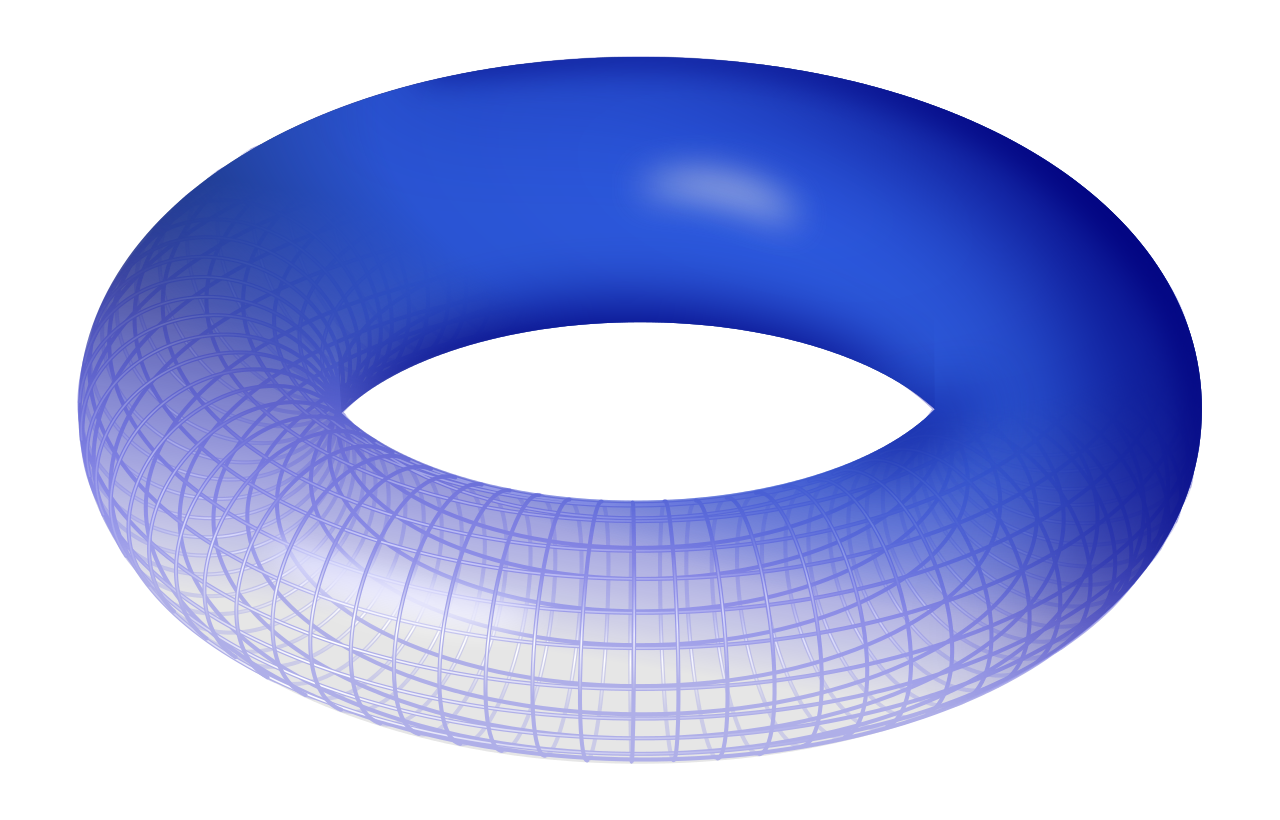
\includegraphics[width=0.5\linewidth]{images/Torus.png}
\caption{Representación clásica de un toro. Imagen extraída de \cite{Wikipedia:Torus}.}
\end{figure}

La expresión paramétrica de un toro es
\begin{equation}
\begin{tabular}{c c l}
$x$ & $=$ & $r \cos u \cos t + R \cos t$, \\
$y$ & $=$ & $r \cos u \sin t + R \sin t$, \\
$z$ & $=$ & $r \sin u$.
\end{tabular}
\nonumber
\end{equation}

Si renombramos esta expresión como
\begin{equation}\label{Uhlir03-14}
c_u = \cos u, \hspace{0.5cm} c_t = \cos t, \hspace{0.5cm} s_u = \sin u \hspace{0.5cm} \text{y} \hspace{0.5cm} s_t = \sin t,
\end{equation}
podemos representar la expresión paramétrica inicial en polinomios como
\begin{equation}\label{Uhlir03-15}
\begin{tabular}{r c c}
$x - r c_u c_t - R c_t$ & $=$ & $0$, \\
$y - r c_u s_t - R s_t$ & $=$ & $0$, \\
$z - r s_u$ & $=$ & $0$.
\end{tabular}
\end{equation}
Añadiendo las identidades
\begin{equation}
\begin{tabular}{r c c}
$c_u^2 + s_u^2 - 1 = 0$ & $=$ & $0$, \\
$c_t^2 + s_t^2 - 1 = 0$ & $=$ & $0$.
\end{tabular}
\end{equation}
La base de Gröbner reducida para el ideal $I$, generado por los polinomios (\ref{Uhlir03-14}) y (\ref{Uhlir03-15}), contiene 9 elementos. Uno solo de estos elementos no contiene variables en $c_u, s_u, c_t \text{ ó } s_t$, y tiene la forma
$$(x^2 + y^2 + z^2 - r^2 - R^2)^2 = 4 R^2 (z^2 - r^2),$$
la cual es la expresión implícita del toro.

\subsection{Método de la resultante}

El término { \em resultante} se suele introducir si se presenta la siguiente cuestión: ¿Cuándo dos polinomios en el anillo de polinomios $K[x]$ tienen un divisor común? Los métodos que usan la evaluación de la resultante se pueden usar para eliminar un subconjunto de variables del sistema inicial de ecuaciones algebraicas no lineales.
Un dato interesante de la resultante para polinomios en varias variables es que para $n+1$ polinomios ésta elimina $n$ variables a la par. A diferencia del método de la base de Gröbner, este método es no secuencial. La idea básica que subyace en las resultantes multidimensionales es la conversión de un problema de eliminación no lineal en uno lineal, lo cual ayuda a aplicar métodos conocidos de Álgebra Lineal para resolver el sistema.

Existen distintos tipos de resultante. La definición básica involucra dos polinomios en una variable, por ejemplo la resultante de Sylvester o Bézout, y a partir de ahí se puede ir generalizando a dos polinomios en dos variables y después a tres polinomios en dos variables, la resultante de Dixon. Esta última puede generalizarse a $n+1$ polinomios en $n$ variables. Aquí daremos una simple pincelada para dar la idea de las resultantes ya nombradas. Podemos encontrar más información en \cite{Berchtold00}.

\subsubsection*{Resultante de Sylvester}

El principal problema es la tendencia a encontrar si dos polinomios $f, g \in K[x]$ tienen divisor común. Existen varias maneras de encontrarlo, por ejemplo, el algoritmo de Euclides se puede usar para descomponer los polinomios en productos de factores simples. O por ejemplo, el siguiente lema.

\begin{lemma}
	Sean $f,g \in K[x]$ tales que $deg(f) = n > 0$ y $deg(g) = m > 0$. Se tiene que $f$ y $g$ tienen un divisor común si y sólo si existen polinomios $A, B \in K[x]$ verificando que
	\begin{enumerate}
		\item ambos polinomios $A$ y $B$ son no nulos,
		\item $A$ y $B$ tienen como mínimo grado $m-1$ y $n-1$ respectivamente y
		\item $Af + Bg = 0$.
	\end{enumerate}
\end{lemma}

\begin{definition}
	Sean $f, g \in K[x]$ dados como $f = a_n x^n + \dots + a_0$ y $g = b_m x^m + \dots + b_0$ donde $a_n, b_m \neq 0$, entonces la resultante de Sylvester de $f$ y $g$ es de la forma
$$\operatorname{Res}(f,g) = \operatorname{Det}(\operatorname{Syl}(f,g)).$$
Donde $\operatorname{Syl}(f,g)$ denota
	$$\begin{pmatrix}
	a_n & & & & & b_m & & & & \\
	a_{n-1} & a_n & & & & b_{m-1} & b_m & & & \\
	a_{n-2} & a_{n-1} & a_n & & & b_{m-2} & b_{m-1} & b_m & & \\
	\vdots & \vdots & & \ddots & \vdots & \vdots & \vdots & \vdots & \ddots & \\
	a_1 & \dotso & \dotso & \dotso & a_{n} & b_1 & \dotso & \dotso & \dotso & b_{m} \\
	a_0 & \dotso & \dotso & \dotso & a_{n-1} & b_0 & \dotso & \dotso & \dotso & b_{m-1} \\
	 & a_0 & \dotso & \dotso & a_{n-2} & & b_0 & \dotso & \dotso & b_{m-2} \\
	 & & \ddots & \vdots & \vdots & & & \ddots & \vdots & \vdots \\
	 & & & a_1 & a_0 & & & & b_1 & b_0 \\
	 & & & & a_0 & & & & & b_0
	\end{pmatrix}$$
y los espacios en blanco de la matriz denotan ceros.
\end{definition}

Ahora realizaremos un ejemplo sencillo para comparar este método con el de la base de Gröbner.

Sean por ejemplo los polinomios en la variable $x$ cuyos coeficeintes son polinomios en la variable $y$
$$f = x^2 y - 1, \hspace{2cm} g = x^2 + y^2 + xy - 4.$$

Aplicando el método de la resultante de Sylvester tenemos
$$\operatorname{Res}(f,g) = \operatorname{Det} \begin{pmatrix}
y & 0 & 1 & 0 \\
0 & y & y & 1 \\
-1 & 0 & y^2 - 4 & y \\
0 & -1 & 0 & y^2 - 4
\end{pmatrix} = y^6 - 8y^4 + y^3 + 16y^2 - 8y + 1.$$

Para comparar podemos ver la solución obtenida mediante el método de la base de Gröbner para el ideal $I = \langle f,g \rangle$ cuya base de Gröbner reducida respecto del orden lexicográfico sería
$$\langle x - 4y^5- y^4 + 32y^3 + 4y^2 - 64y + 16 , y^6 - 8y^4 + y^3 + 16y^2 - 8y + 1 \rangle.$$

\subsubsection*{Resultante de Bézout}

Es similar a la resultante de Sylvester, salvo que la definición de matriz de Bézout es un poco más dificultosa que ésta, pero a cambio ésta tiene dimensión $n \times n$ en lugar de la dimensión $(n+m) \times (n+m)$. En consecuencia, la evaluación del determinante de la matriz Bézout es mucho más rápido.

\subsubsection*{Resultante de Dixon}

Es una versión generalizada de la resultante y matriz de Bézout para tres polinomios en dos variables. Entonces la resultante de Dixon se generaliza para $n+1$ polinomios en $n$ variables.

\subsection{El método de Wu-Ritt}

En esta sección daremos una breve introducción a la teoría de este método. Éste se basa en la aproximación de Wu-Ritt para encontrar un conjunto característico para un sistema de ecuaciones no lineales. Dado un sistema de ecuaciones polinomiales $S = \{ f_1, \dotso, f_m \}$ se transforma en una forma triangular $S'$. Es importante notar que si el número $n$ de variables es mayor que el número de ecuaciones del conjunto $S$, entonces el conjunto de variables se divide en dos subconjuntos: las variables independientes, que denotaremos por $\{ u_1, \dotso, u_k \}$, y las dependientes, que denotaremos por $\{ y_1, \dotso, y_l \}$.

La pseudodivisión de polinomios de varias variables es la operación clave en la computación de conjuntos característicos. Para realizar la pseudodivisión se da uso de la representación recursiva de los polinomios con lo cual se define la siguiente reducción polinomial.

Un polinomio $f_i$ se reduce respecto de otro polinomio $f_j$ si verifican una de las dos siguientes condiciones:
\begin{enumerate}
\item La mayor variable de $f_i$ es menor, con respecto a $\prec$ , que la mayor variable de $f_j$.
\item El grado de la mayor variable en $f_j$ es mayor que el grado de la mayor variable en $f_i$.
\end{enumerate} 

Si $f_i$ no es reducible respecto de $f_j$, entonces $f_i$ se reduce a $r$ mediante la pseudodivisión entre $f_j$.

\begin{definition}
	Dado un conjunto finito $\Sigma$ de polinomios $u_1, \dotso, u_k, y_1, \dotso, y_l$ un conjunto característico $\Phi$ de $\Sigma$ se define de cualquiera de las siguientes maneras:
	\begin{enumerate}
		\item $\{ g_1 \}$ donde $g_1$ es un polinomio de $\{ u_1, \dotso, u_k \}$.
		\item Una cadena $\langle g_1, \dotso, g_l \rangle$ donde cada $g_i$ es un polinomio en $\{ u_1, \dotso, u_k, y_1, \dotso, y_i \}$, con coeficiente líder $LC(g_i)$, tales que:
		\begin{itemize}
			\item Cualquier cero de $\Sigma$ es un cero de $\Phi$.
			\item Cualquier cero de $\Phi$ que no es cero de ninguno de los coeficientes líderes $LC(g_i)$ es un cero de $\Sigma$.
		\end{itemize}
	\end{enumerate}
\end{definition}
Podemos encontrar más información sobre el presente método en \cite{Berchtold00}, \cite{Gallo91_2} o \cite{Gallo91_1}.

\section{Conclusiones}

Todos los métodos mencionados tienen una característica común: si hacemos uso de ellos para convertir la expresión paramétrica de un objeto a la expresión implícita de éste entonces lo que obtenemos es una sola ecuación. A partir de ahí las superficies pueden ser visualizadas con métodos de visualización directa.

Por supuesto, esto es solo un tipo de métodos de implicitación de superficies, ya que existe una  gran variedad. Alguno ya ha sido mencionado al comienzo de este capítulo y otros pueden ser consultados en la bibliografía. En este tipo de métodos no es necesario conocer la expresión paramétrica del objeto.